\section{Практычны занятак №2}

\subsection{Структура праекта}

На малюнку \ref{img: pz2} прадстаўлена файлавая структура праекта.

\begin{figure}[h!]
    \centering
    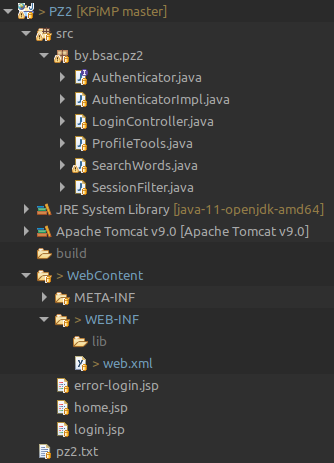
\includegraphics[width=0.5\textwidth]{pz2_structure}
    \caption{Файлавая структура практычнага занятку}
    \label{img: pz2} 
\end{figure}

\vspace{-\baselineskip}
\subsection{Заданне з тэорыі}

\subsubsection{Апіанне задання.}

Стварыць вэб-праграму, якая перанакіроўвае любы URL-адрас
на старонку \textit{login}, дзе карыстальніку неабходна
прайсці аўтэнтыфікацыю. Пры паспяховаў аўтэнтыфікацыі вывесці
старонку \textit{home}, пры памылцы ў логіну альбо паролі ---
вывесці старонку \textit{error-login}.

\subsection{Зыходны код. JSP-старонкі}

У лістынку \ref{lst: pz2_error-login} прадстаўлена старонка
\textit{error-login.jsp}.

\lstinputlisting[caption={Зыходны код для error-login},%
                 label={lst: pz2_error-login},%
                 language=HTML5,%
                 style=htmlcssjs]{PZ2/JSP/error-login.jsp}

У лістынку \ref{lst: pz2_home} прадстаўлена старонка
\textit{home.jsp} з дадатковымі тлумачэннямі.

\lstinputlisting[caption={Зыходны код для home},%
                 label={lst: pz2_home},%
                 language=HTML5,%
                 style=htmlcssjs]{PZ2/JSP/home.jsp}

У лістынку \ref{lst: pz2_login} прадстаўлена старонка
\textit{login.jsp} з дадатковымі тлумачэннямі.

\lstinputlisting[caption={Зыходны код для login},%
                 label={lst: pz2_login},%
                 language=HTML5,%
                 style=htmlcssjs]{PZ2/JSP/login.jsp}

\subsection{Зыходны код. Java}

\subsubsection{Клас ProfileTools.}

Клас \textit{ProfileTools} з'яўляецца дапаможным класам.
Ён захоўвае імёны атрыбутаў сесіі, якія ўстанаўліваюцца
падчас работы вэб-праграмы, а таксама метад
\textit{isLoggedIn} для праверкі статусу карыстальніка.

У лістынгу \ref{lst: pz2_profileTools} прадстаўлены зыходны код класа \textit{ProfileTools}.

\lstinputlisting[caption={Зыходны код класа ProfileTools},%
                 label={lst: pz2_profileTools},%
                 language=java]{PZ2/Java/ProfileTools.java}

\subsubsection{Інтэрфейс Authenticator.}

Інтэрфейс \textit{Authenticator} вызначае метады, якія маюць
быць вызначаны ў класе \textit{Au\-then\-ti\-ca\-tor\-Impl}.

У лістынгу \ref{lst: pz2_authenticator} прадстаўлены зыходны код інтэрфейса \textit{Authenticator}.

\lstinputlisting[caption={Зыходны код інтэрфейса Authenticator},%
                 label={lst: pz2_authenticator},%
                 language=java]{PZ2/Java/Authenticator.java}

\subsubsection{Клас AuthenticatorImpl.}

Клас \textit{AuthenticatorImpl} захоўвае інфармацыю для ўваходу ў
вэб-праграму, рэалізуе праверку ўведзеных даных з данымі доступу.

У лістынгу \ref{lst: pz2_authenticatorImpl} прадстаўлены зыходны код класа \textit{AuthenticatorImpl}.

\lstinputlisting[caption={Зыходны код класа AuthenticatorImpl},%
                 label={lst: pz2_authenticatorImpl},%
                 language=java]{PZ2/Java/AuthenticatorImpl.java}

\subsubsection{Клас LoginController}

Клас \textit{LoginController} з'яўляецца сервлетам
вэб-праграмы, які прапаноўвае старонку для аўтэнтыфікацыі
і адказвае за выкананне аўтэнтыфікацыі:
праверка ўведзеных даных з правільнымі,
перанапраўленне на адпаведную старонку пры аўтэнтыфікацыі.

У лістынгу \ref{lst: pz2_loginController} прадстаўлены зыходны код класа \textit{LoginController}.

\lstinputlisting[caption={Зыходны код класа LoginController},%
                 label={lst: pz2_loginController},%
                 language=java]{PZ2/Java/LoginController.java}

\subsection{Зыходны код. web.xml}

